\chapter{The Litwin-Kumar and Doiron Baseline}
\label{ch:litwin-kumar-doiron-baseline}

\textit{The baseline model for this rotation is a balanced spiking network with clustered excitatory connectivity. The random balanced network supplies fast asynchronous irregular spiking. Excitatory clustering adds slow cluster up-states and down-states. Finite-size fluctuations then move the network among many metastable activity patterns.}

\begin{aside}[Citation TODO]
Resolve the exact bibliography entry for the Litwin-Kumar and Doiron clustered balanced network paper before adding a \texttt{\textbackslash cite} command. The discussion below uses only the safe mechanism-level description: excitatory clustering inside a balanced spiking network creates attractor-like cluster states and slow variability.
\end{aside}

% ============================================================
\section{Balanced E/I networks as the starting point}
\label{sec:balanced-ei-networks-starting-point}
% ============================================================

The starting point is not a pure attractor network. It is a balanced excitation--inhibition network in which excitatory and inhibitory inputs are individually large but nearly cancel. This matters because the model should produce irregular spiking even before clustering is added.

For a current-based spiking network, a compact microscopic description is
%
\begin{equation}
  \tau_m \frac{\dd V_i}{\dd t}
  =
  -(V_i-V_L)
  +
  R_m\left[
    I_i^{\mathrm{ext}}(t)
    +
    \sum_{j=1}^N J_{ij}x_j(t)
  \right],
  \label{eq:lkd-membrane-current}
\end{equation}
%
with threshold and reset. Here $V_i$ is the membrane potential, $V_L$ is the leak reversal level, $R_m$ is membrane resistance, $I_i^{\mathrm{ext}}$ is external drive, $J_{ij}$ is the signed synaptic weight from neuron $j$ to neuron $i$, and $x_j(t)$ is a filtered version of the presynaptic spike train.

The filtered synaptic variable may be written as
%
\begin{equation}
  \tau_s \dot x_j
  =
  -x_j+s_j(t),
  \qquad
  s_j(t)=\sum_m\delta(t-t_j^m).
  \label{eq:lkd-synaptic-filter}
\end{equation}
%
The spike train $s_j$ is a sum of impulses. The synaptic filter $x_j$ converts those impulses into postsynaptic current with time scale $\tau_s$.

Balance is a statement about the total input,
%
\begin{equation}
  I_i^{E}(t)+I_i^{I}(t)+I_i^{\mathrm{ext}}(t)
  =
  O(1),
  \qquad
  |I_i^{E}(t)|,\ |I_i^{I}(t)| \gg 1
  \quad
  \text{in network units}.
  \label{eq:balanced-cancellation}
\end{equation}
%
$I_i^E$ is the excitatory recurrent current. $I_i^I$ is the inhibitory recurrent current. The residual is small enough that neurons remain in a fluctuation-driven spiking regime rather than saturating at unrealistically high rates.

The practical baseline is therefore: first reproduce an unclustered balanced network with plausible rates, irregular single-neuron spiking, and no slow cluster-like structure. Clustering should be added only after this baseline is working.

% ============================================================
\section{Random balanced networks and asynchronous irregular activity}
\label{sec:random-balanced-networks-ai-activity}
% ============================================================

In a random balanced network, connections are drawn without cluster structure. Let $a,b\in\{E,I\}$ denote postsynaptic and presynaptic cell classes. If a neuron of class $a$ receives on average $K_{ab}$ inputs from class $b$, each with synaptic amplitude $J_{ab}$, then a mean-field estimate of the input mean is
%
\begin{equation}
  \mu_a
  =
  I_a^{\mathrm{ext}}
  +
  \sum_{b\in\{E,I\}} K_{ab}J_{ab}r_b .
  \label{eq:balanced-mean-input}
\end{equation}
%
$r_b$ is the mean firing rate of class $b$. Excitatory weights have positive sign and inhibitory weights have negative sign, or equivalently inhibition is represented by subtracting a positive inhibitory term. Balance means the excitatory and inhibitory contributions nearly cancel in $\mu_a$.

The same inputs also produce fluctuations. Under a simple independent-input approximation,
%
\begin{equation}
  \sigma_a^2
  =
  \sum_{b\in\{E,I\}}
  K_{ab}J_{ab}^2r_b
  \int_0^\infty \kappa_{ab}^2(t)\,\dd t .
  \label{eq:balanced-input-variance}
\end{equation}
%
The mean uses signed weights $J_{ab}$, so excitation and inhibition can cancel. The variance uses squared weights $J_{ab}^2$, so excitatory and inhibitory events both add positive fluctuation power.

\begin{keyequation}[Balanced Irregular Operating Point]
\begin{equation}
  \text{large } E \text{ current}
  \;+\;
  \text{large } I \text{ current}
  \;\approx\;
  \text{small fluctuating residual}.
  \label{eq:balanced-operating-point}
\end{equation}
\tcblower
The residual input is small in mean but noisy in time. This produces irregular spikes without requiring slow attractor switching.
\end{keyequation}

Asynchronous irregular activity means two things. ``Irregular'' means individual neurons fire with variable interspike intervals, often with CV near one. ``Asynchronous'' means the population does not fire in large synchronized volleys; pairwise correlations and population-rate oscillations remain limited in the unstructured baseline.

This unclustered network is a control. If it already shows very slow metastability, then clustering is not the explanation. If it is irregular but lacks slow state switching, then adding clustered excitation has a clear mechanistic role.

% ============================================================
\section{Adding clustered excitatory connectivity}
\label{sec:adding-clustered-excitatory-connectivity}
% ============================================================

Excitatory clustering partitions excitatory neurons into $K$ groups,
%
\begin{equation}
  \mathcal{C}_1,\ldots,\mathcal{C}_K,
  \qquad
  \mathcal{C}_k\cap \mathcal{C}_\ell=\varnothing\ (k\ne \ell),
  \qquad
  \bigcup_{k=1}^K \mathcal{C}_k=\{1,\ldots,N_E\}.
  \label{eq:excitatory-cluster-partition}
\end{equation}
%
The clusters are not anatomical objects in the first instance. They are structured recurrent assemblies in the model. Neurons inside the same cluster have stronger or more probable recurrent excitation than neurons in different clusters.

A standard schematic parameterization is
%
\begin{equation}
  J_{ij}^{EE}
  =
  \begin{cases}
    J_+J_{EE}, & i,j\in \mathcal{C}_k \text{ for the same } k,\\
    J_-J_{EE}, & i\in \mathcal{C}_k,\ j\in \mathcal{C}_\ell,\ k\ne \ell,
  \end{cases}
  \label{eq:clustered-ee-weights}
\end{equation}
%
where $J_+>1$ strengthens within-cluster excitation and $J_-<1$ weakens between-cluster excitation. The exact implementation may cluster connection probabilities, synaptic weights, or both. The mesoscopic consequence is the same: activity in a cluster feeds back more strongly onto that same cluster than onto other clusters.

Often one keeps the average recurrent excitation approximately fixed while changing cluster strength. If $f_{\mathrm{in}}$ is the fraction of recurrent excitatory partners drawn from the same cluster, a simple normalization is
%
\begin{equation}
  f_{\mathrm{in}}J_+
  +
  (1-f_{\mathrm{in}})J_-
  =
  1.
  \label{eq:cluster-normalization}
\end{equation}
%
This equation says that clustering redistributes recurrent excitation rather than merely increasing all excitation. Increasing $J_+$ then forces $J_-$ downward. The network becomes more modular without changing the mean excitatory scale as much.

\begin{figure}[h]
\centering
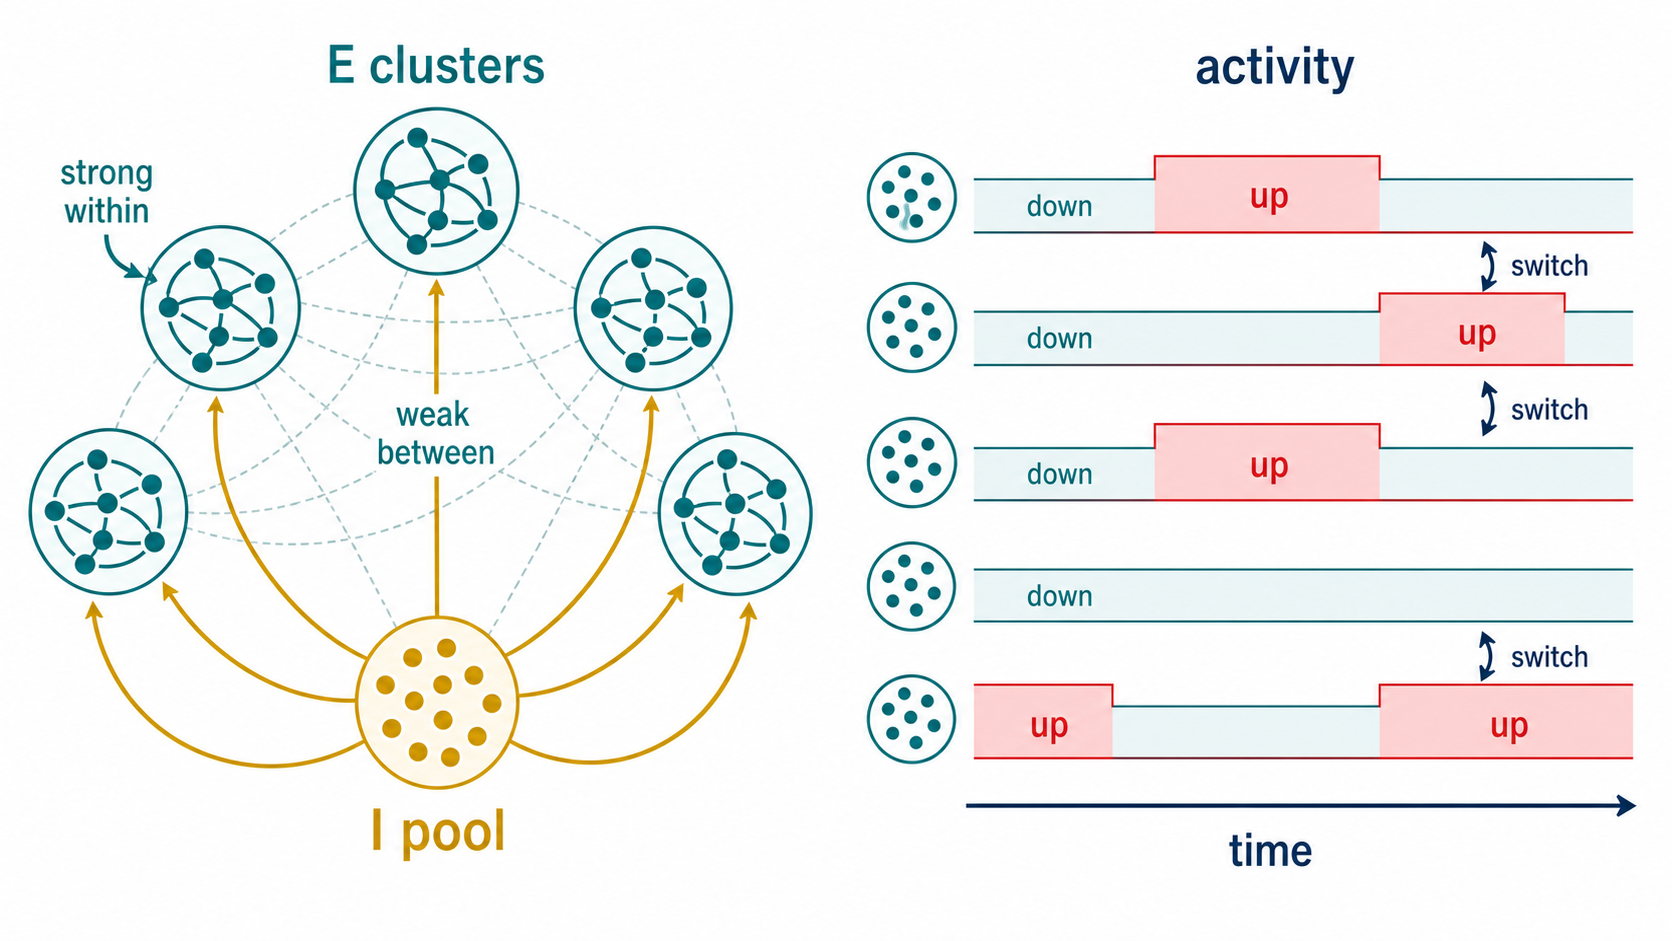
\includegraphics[width=0.95\textwidth]{figures/meso-lkdoiron-clustered-balanced-network.png}
\caption{The clustered balanced network keeps the E/I background but makes recurrent excitation stronger inside excitatory clusters than between them. This creates cluster-level up and down states: active clusters can persist for a while, then switch as finite-size fluctuations and inhibition reshape the effective input.}
\label{fig:lkdoiron-clustered-balanced-network}
\end{figure}

The important control parameter is not the absolute value of one synapse. It is the effective recurrent gain of a cluster: how much an increase in cluster activity feeds back into further activity of the same cluster.

% ============================================================
\section{Cluster up-states and down-states}
\label{sec:cluster-up-states-down-states}
% ============================================================

For each excitatory cluster, define a smoothed cluster rate
%
\begin{equation}
  r_k(t)
  =
  \frac{1}{N_k}\sum_{i\in\mathcal{C}_k}(\kappa*s_i)(t),
  \label{eq:lkd-smoothed-cluster-rate}
\end{equation}
%
where $N_k=|\mathcal{C}_k|$ and $\kappa$ is a smoothing or synaptic kernel. $r_k(t)$ measures the population output of cluster $k$.

A cluster is in an up-state when $r_k(t)$ is high enough that recurrent excitation within the cluster helps maintain the high activity. It is in a down-state when the cluster has low activity and receives insufficient net excitation to turn on. A binary detection variable is
%
\begin{equation}
  m_k(t)
  =
  \mathbf{1}\{r_k(t)>\theta_{\mathrm{up}}\},
  \label{eq:cluster-up-indicator}
\end{equation}
%
where $\theta_{\mathrm{up}}$ is an analysis threshold. The threshold is not part of the microscopic model; it is part of the state-detection protocol.

A mesoscopic input equation makes the mechanism transparent:
%
\begin{equation}
  u_k(t)
  =
  h_k(t)
  +
  J_+ r_k(t)
  +
  J_-\sum_{\ell\ne k} r_\ell(t)
  -
  J_{EI}r_I(t).
  \label{eq:cluster-effective-input}
\end{equation}
%
$h_k$ is external drive. $J_+r_k$ is recurrent self-excitation. $J_-\sum_{\ell\ne k}r_\ell$ is between-cluster excitation. $J_{EI}r_I$ is shared inhibition. Varying $J_+$ changes how self-sustaining an up-state can be. Varying inhibition changes how many clusters can be active together.

The up/down language is useful only if it is tied to measurements. In a simulation one should compute cluster-rate histograms, check for separated low and high modes, define a fixed threshold, and report cluster lifetimes under that detection rule.

% ============================================================
\section{Bistability and metastability}
\label{sec:bistability-and-metastability}
% ============================================================

Bistability means that two stable states coexist for the same parameters. In a clustered network, the simplest local form is coexistence of a low-rate and high-rate state for one cluster, after treating the rest of the network as an effective input.

Consider a one-cluster reduction
%
\begin{equation}
  \tau \dot r
  =
  -r+\Phi(wr+I_{\mathrm{eff}}).
  \label{eq:one-cluster-bistability}
\end{equation}
%
$r$ is the cluster rate, $\tau$ is the relaxation time, $\Phi$ is the input--output function of the clustered population, $w$ is effective recurrent self-excitation, and $I_{\mathrm{eff}}$ includes external drive, inhibition, and background input from other clusters.

Fixed points satisfy
%
\begin{equation}
  r^*
  =
  \Phi(wr^*+I_{\mathrm{eff}}).
  \label{eq:one-cluster-fixed-point}
\end{equation}
%
If the graph of $\Phi(wr+I_{\mathrm{eff}})$ crosses the line $r$ three times, the lower and upper crossings can be stable while the middle crossing is unstable. The low stable crossing is the down-state. The high stable crossing is the up-state. The middle crossing acts as a separatrix in this one-dimensional picture.

The saddle-node condition for creating or destroying the pair of fixed points is
%
\begin{keyequation}[Up-State Bifurcation Condition]
\begin{equation}
  r^*
  =
  \Phi(wr^*+I_{\mathrm{eff}}),
  \qquad
  1
  =
  w\,\Phi'(wr^*+I_{\mathrm{eff}}).
  \label{eq:upstate-saddle-node-condition}
\end{equation}
\tcblower
The first equation says the rate is self-consistent. The second says recurrent gain exactly balances the leak at the tangent point.
\end{keyequation}

\noindent Metastability is different from bistability. Bistability describes the deterministic skeleton: multiple stable states exist. Metastability describes the observed finite network: the system spends long times near one state but eventually leaves it.

With many clusters, the deterministic state can be indexed by an active set
%
\begin{equation}
  \mathcal{S}(t)
  =
  \{k:\ r_k(t)>\theta_{\mathrm{up}}\}.
  \label{eq:active-cluster-set}
\end{equation}
%
Different active sets are different attractor-like states. The network is metastable when $\mathcal{S}(t)$ persists for a while, then changes.

% ============================================================
\section{Finite-size noise as a switching mechanism}
\label{sec:finite-size-noise-switching-mechanism}
% ============================================================

The baseline mechanism does not require externally imposed slow noise. A finite cluster contains finitely many neurons, so its population activity fluctuates. Those fluctuations can push the cluster rate across the boundary between basins.

For a cluster of size $N_k$, define a binned empirical activity
%
\begin{equation}
  \widehat A_k(t;\Delta t)
  =
  \frac{1}{N_k\Delta t}
  \sum_{i\in\mathcal{C}_k}
  N_i(t,t+\Delta t).
  \label{eq:cluster-binned-activity}
\end{equation}
%
If neurons were conditionally independent Poisson processes with common rate $r_k(t)$ within the bin, then
%
\begin{equation}
  \E[\widehat A_k(t;\Delta t)]=r_k(t),
  \qquad
  \Var[\widehat A_k(t;\Delta t)]
  =
  \frac{r_k(t)}{N_k\Delta t}.
  \label{eq:cluster-activity-finite-size-variance}
\end{equation}
%
The standard deviation scales like $N_k^{-1/2}$. Larger clusters average away private spiking noise more effectively. Correlations can weaken this scaling, so the formula is a baseline to test rather than a guarantee.

A mesoscopic switching model writes
%
\begin{equation}
  \dd r_k
  =
  f_k(\vec r)\,\dd t
  +
  \frac{1}{\sqrt{N_k}}g_k(\vec r)\,\dd W_k(t),
  \label{eq:cluster-finite-size-langevin}
\end{equation}
%
where $f_k$ is deterministic drift, $g_k$ is state-dependent noise amplitude, and $W_k$ is Brownian motion. The noise term is multiplicative because spike-count variance depends on current activity.

For escape over a barrier, a large-deviation intuition is
%
\begin{equation}
  \E[L_k]
  \approx
  A(\theta)\exp\!\left(N_k\Delta S(\theta)\right).
  \label{eq:cluster-dwell-large-deviation}
\end{equation}
%
$L_k$ is a dwell time, $A(\theta)$ is a prefactor depending on parameters, and $\Delta S(\theta)$ is an effective action or barrier. The crucial prediction is the exponential sensitivity to cluster size. If the finite-size escape picture is correct, increasing $N_k$ should strongly lengthen lifetimes after deterministic parameters are matched.

The next simulation task is therefore not only to observe switches. It is to repeat the observation at different cluster sizes and ask whether dwell times scale as a finite-size noise theory predicts.

% ============================================================
\section{Why clustered networks produce slow dynamics}
\label{sec:why-clustered-networks-produce-slow-dynamics}
% ============================================================

The microscopic model contains fast membrane and synaptic time constants, yet the clustered network can show much slower activity fluctuations. The slowness comes from collective state structure.

There are two complementary views. The first is linear stability near a state. If $\vec r^*$ is a cluster-state fixed point and $\delta\vec r=\vec r-\vec r^*$, then
%
\begin{equation}
  \frac{\dd}{\dd t}\delta\vec r
  =
  \Jac(\vec r^*)\,\delta\vec r .
  \label{eq:cluster-linearization}
\end{equation}
%
Eigenvalues of $\Jac$ with real parts close to zero create slow relaxation. A perturbation along such an eigenmode decays only gradually. Clustered recurrence can tune some modes near this boundary because self-excitation nearly cancels leak.

The second view is state switching. Suppose a coarse cluster state alternates between $A$ and $B$ with transition rates $q_{A\to B}$ and $q_{B\to A}$. The autocorrelation time of the two-state indicator is
%
\begin{equation}
  \tau_{\mathrm{state}}
  =
  \frac{1}{q_{A\to B}+q_{B\to A}}.
  \label{eq:two-state-autocorrelation-time}
\end{equation}
%
If transitions are rare, $\tau_{\mathrm{state}}$ is long even though spikes inside each state are fast and irregular.

This is why clustered networks are useful for variability. They can separate two time scales: millisecond spike irregularity inside a state, and hundreds-of-milliseconds or longer fluctuations in which cluster state is occupied. The latter is what inflates long-window Fano factors and low-frequency power.

% ============================================================
\section{How stimuli bias the network into fewer states}
\label{sec:stimuli-bias-network-fewer-states}
% ============================================================

A stimulus can be modeled as a structured input to clusters:
%
\begin{equation}
  h_k(t)
  =
  h_0+\Delta h_k(t).
  \label{eq:stimulus-cluster-input}
\end{equation}
%
$h_0$ is baseline drive. $\Delta h_k$ is the stimulus-specific bias. Positive $\Delta h_k$ makes cluster $k$ more likely to enter or remain in an up-state; negative or indirect inhibitory effects can make other clusters less likely to be active.

At the active-set level, the stimulus changes the occupancy distribution
%
\begin{equation}
  P_{\mathrm{spont}}(\mathcal{S})
  \quad\longrightarrow\quad
  P_{\mathrm{evoked}}(\mathcal{S}\mid \text{stimulus}).
  \label{eq:state-occupancy-stimulus}
\end{equation}
%
In spontaneous activity, probability may be spread across many active sets. After stimulus onset, probability may concentrate on a smaller set of stimulus-compatible active sets.

This gives a mechanistic route to variability quenching. If the spike count depends on the active set through $\mu_{\mathcal{S}}=\E[N\mid \mathcal{S}]$, then
%
\begin{equation}
  \Var[\mu_{\mathcal{S}}]_{\mathrm{evoked}}
  <
  \Var[\mu_{\mathcal{S}}]_{\mathrm{spont}}
  \quad
  \Rightarrow
  \quad
  F_{\mathrm{evoked}}(T)<F_{\mathrm{spont}}(T)
  \label{eq:stimulus-quenching-state-variance}
\end{equation}
%
after controlling for mean-count changes. The stimulus does not need to eliminate irregular spiking. It needs to reduce uncertainty about the slow latent state.

The most direct analysis is to measure $P(\mathcal{S})$, the entropy or dimensionality of cluster activity, and the Fano factor before and after stimulus onset. The clustered-network hypothesis predicts that these quantities should change together.

% ============================================================
\section{What the 2012 model explains well}
\label{sec:model-explains-well}
% ============================================================

The Litwin-Kumar--Doiron-style baseline is valuable because it links several observations with one circuit mechanism.

First, it explains how a network can have irregular single-neuron spiking and slow population variability at the same time. Balance provides fluctuation-driven spiking. Clustering provides slow collective state changes.

Second, it explains super-Poisson spike counts without requiring every neuron to be intrinsically bursty. Slow transitions among cluster states change the integrated rate across windows and trials, adding the $\Var[\Lambda_T]$ term in the Fano factor.

Third, it gives a concrete state variable for variability quenching. Stimuli can bias the network into a smaller set of cluster configurations, reducing across-trial latent-state variance while preserving irregular spiking inside the selected states.

Fourth, it predicts structured correlations. Neurons in the same active cluster should share slow rate fluctuations. Competing clusters can show anticorrelated activity if shared inhibition limits the number of active clusters.

Fifth, it creates reproducible analysis targets:
%
\begin{equation}
  r_k(t),
  \qquad
  n_{\mathrm{act}}(t),
  \qquad
  F(T),
  \qquad
  \rho_{r_k}(\tau),
  \qquad
  S_L(t)=\mathbb{P}\{L>t\}.
  \label{eq:lkd-reproduction-targets}
\end{equation}
%
These are cluster rates, active-cluster count, Fano factor, cluster-rate autocorrelation, and lifetime survival. They form the minimum bridge from microscopic simulation to mesoscopic theory.

For the rotation, this model is the E-only control. Any E/I clustered extension should be judged against what this baseline already explains.

% ============================================================
\section{What it leaves open}
\label{sec:model-leaves-open}
% ============================================================

The baseline also leaves open exactly the questions that motivate the course.

First, it does not by itself provide a closed mesoscopic theory. The microscopic simulation can show cluster switching, but the rotation needs equations for the cluster variables, their fixed points, their stability, and their finite-size noise.

Second, the mechanism can be parameter sensitive. If within-cluster excitation is too weak, up-states disappear. If it is too strong, clusters can become unrealistically persistent or drive pathological synchrony. The useful regime lies between these failures.

Third, inhibition is often treated as a shared pool rather than a structured partner to each excitatory cluster. This makes E-only clustering a clean baseline but may limit robustness. The Rostami-style E/I extension asks whether local inhibitory clustering can preserve metastability while improving balance and widening the viable parameter regime.

Fourth, finite-size switching and deterministic irregular population dynamics can look similar in rasters. A slow cluster-rate trace alone does not prove noise-driven escape. One needs scaling tests, perturbation tests, and mesoscopic stability analysis.

Fifth, exact citation-dependent details must be checked against the source paper before the final notes make historical or parameter-specific claims. The safe model-building takeaway is the mechanism: balanced irregular spiking plus structured excitatory recurrence yields metastable cluster dynamics.

The next chapter path is therefore clear. Build the spiking-network foundations, define balanced and clustered architectures precisely, then reduce the clustered dynamics to mesoscopic variables whose deterministic and stochastic terms can be analyzed.

\begin{chaptersummary}

\begin{center}
\renewcommand{\arraystretch}{1.55}
\begin{tabularx}{\textwidth}{@{}l X X@{}}
  \toprule
  \textbf{Mechanism} & \textbf{Equation or object} & \textbf{Interpretation} \\
  \midrule
  Microscopic spiking &
  $\tau_m\dot V_i=-(V_i-V_L)+R_m(I_i^{\mathrm{ext}}+\sum_jJ_{ij}x_j)$ &
  Spikes arise from filtered recurrent and external currents \\
  Balance &
  $\mu_a=I_a^{\mathrm{ext}}+\sum_bK_{ab}J_{ab}r_b$ &
  Large E and I currents cancel in the mean residual drive \\
  Input fluctuations &
  $\sigma_a^2=\sum_bK_{ab}J_{ab}^2r_b\int\kappa_{ab}^2$ &
  Squared weights make excitation and inhibition both contribute variance \\
  Excitatory clustering &
  $J_{ij}^{EE}=J_+J_{EE}$ within, $J_-J_{EE}$ between &
  Recurrent excitation is concentrated inside clusters \\
  Cluster state &
  $m_k=\mathbf{1}\{r_k>\theta_{\mathrm{up}}\}$ &
  Up/down states turn population activity into a discrete latent variable \\
  Up-state condition &
  $r^*=\Phi(wr^*+I_{\mathrm{eff}})$, $1=w\Phi'$ &
  A high-rate state appears when recurrent gain balances leak \\
  Finite-size switching &
  $\dd r_k=f_k\,\dd t+N_k^{-1/2}g_k\,\dd W_k$ &
  Finite clusters fluctuate across attractor boundaries \\
  Stimulus bias &
  $P_{\mathrm{spont}}(\mathcal{S})\to P_{\mathrm{evoked}}(\mathcal{S}\mid s)$ &
  Quenching can occur by reducing uncertainty over active cluster sets \\
  \bottomrule
\end{tabularx}
\end{center}

\end{chaptersummary}

\begin{conceptquestions}
  \item Why is the unclustered balanced network the right starting point rather than a deterministic attractor network?
  \item In \cref{eq:balanced-mean-input} and \cref{eq:balanced-input-variance}, why can excitation and inhibition cancel in the mean but not in the variance?
  \item What is the purpose of choosing $J_-<1$ when $J_+>1$ in a clustered excitatory network?
  \item How would you detect cluster up-states from a spike raster without tuning the threshold separately for each parameter point?
  \item Explain geometrically how the equation $r=\Phi(wr+I_{\mathrm{eff}})$ can have both low-rate and high-rate stable solutions.
  \item What finite-size scaling of dwell times would support the escape-over-a-barrier interpretation?
  \item Why can a clustered network produce slow autocorrelation even though membrane and synaptic time constants are fast?
  \item How can a stimulus reduce Fano factor without reducing within-state spike irregularity?
  \item List three observables that should be reproduced before trusting a mesoscopic version of the baseline model.
  \item What does the E-only baseline leave unresolved that motivates adding structured inhibitory clusters?
\end{conceptquestions}

\clearpage
